\documentclass[10pt,journal,compsoc]{IEEEtran}

% ==============================================================================
% Packages
% ==============================================================================
\usepackage[utf8]{inputenc}
\usepackage{amsmath}
\usepackage{amssymb}
\usepackage{booktabs}
\usepackage{graphicx}
\usepackage{url}
\usepackage{hyperref}
\usepackage{tikz}
\usepackage[most]{tcolorbox}
\usepackage{stfloats} % Enhanced placement of double-column floating environments
\usetikzlibrary{positioning, shapes.geometric, arrows.meta, fit, backgrounds}

% Patch default em-dashes after Abstract and Index Terms labels using etoolbox
\usepackage{etoolbox}
\patchcmd{\abstract}{\textbf{\abstractname}---\relax}{\textbf{\abstractname}}{}{}
\patchcmd{\abstract}{\textit{\abstractname}---\relax}{\textit{\abstractname}}{}{}
\patchcmd{\IEEEkeywords}{\textbf{\IEEEkeywordsname}---\relax}{\textbf{\IEEEkeywordsname}}{}{}
\patchcmd{\IEEEkeywords}{\textit{\IEEEkeywordsname}---\relax}{\textit{\IEEEkeywordsname}}{}{}

% Increase line spacing slightly for better readability
\renewcommand{\baselinestretch}{1.08}

% Setup TikZ styles for diagrams
\tikzset{
    base/.style={draw, thick, align=center, minimum height=0.8cm, font=\small},
    box/.style={base, rectangle, fill=blue!10, text width=3cm, rounded corners=3pt},
    greenbox/.style={base, rectangle, fill=green!10, text width=3cm, rounded corners=3pt},
    redbox/.style={base, rectangle, fill=red!10, text width=3cm, rounded corners=3pt},
    orangebox/.style={base, rectangle, fill=orange!10, text width=3cm, rounded corners=3pt},
    arrow/.style={-Latex, thick},
    dashedarrow/.style={-Latex, thick, dashed},
    line/.style={draw, thick}
}

% Setup tcolorbox style for bold cards with compact margins to prevent formula overflow
\newtcolorbox{mathcard}[1][]{
  colback=gray!5,
  colframe=blue!60!black,
  boxrule=1.2pt,
  arc=3pt,
  title=#1,
  fonttitle=\bfseries\color{white},
  coltitle=white,
  halign=center,
  left=2pt,
  right=2pt,
  top=4pt,
  bottom=4pt,
  boxsep=1pt
}

% ==============================================================================
% Document Metadata
% ==============================================================================
\begin{document}

\title{Design and Empirical Evaluation of a Distributed, Zero-Trust Architecture for Long-Term DNS Security and Performance Auditing}

\author{Rabin Mishra\\
\small{Graduate Research Proposal \& System Specification}
}

\markboth{Technical Specification Report,~Vol.~1, No.~1, June~2026}%
{Mishra: Chronos-DNS System Specification}

\IEEEtitleabstractindextext{%
\begin{abstract}
\hfill \\
The global Internet is currently undergoing a critical security transition from legacy, unencrypted Domain Name System (DNS) query resolution over UDP/TCP port 53 to cryptographically secured transport protocols: DNS-over-HTTPS (DoH, RFC 8484) and DNS-over-TLS (DoT, RFC 7858). While encryption prevents passive eavesdropping and query manipulation, it introduces transport-layer and cryptographic handshake overheads that alter latency profiles, connection state lifespans, and reliability. This paper presents \textbf{Chronos-DNS}, a production-ready, cloud-native distributed measurement fabric designed to continuously collect, store, and visualize metrics from standard and encrypted resolver end-points. We detail the engineering lifecycle of this system, demonstrating how asynchronous network polling, relational telemetry persistence, zero-trust network topology (via Cloudflare Tunnels), and containerized git-driven CI/CD deployment work in unison to provide high-resolution, empirical datasets. Our proof-of-concept deployment on AWS EC2, monitored via Prometheus and Grafana, validates that DoT and DoH protocols present distinct performance trade-offs, making this measurement framework highly relevant to long-term internet engineering research, such as that conducted by the WIDE Project, CAIDA, and RIPE NCC.
\end{abstract}

\begin{IEEEkeywords}
\hfill \\
\begin{tabular}{lll}
\toprule
\textbf{Core Protocols} & \textbf{Measurement Systems} & \textbf{Operations \& Methodology} \\
\midrule
Domain Name System & Asynchronous Concurrency & GitOps \\
DNS-over-HTTPS (DoH) & Telemetry Architecture & MLOps \\
DNS-over-TLS (DoT) & Zero-Trust Networks & Internet Measurement \\
\bottomrule
\end{tabular}
\vspace{0.6em}
\end{IEEEkeywords}}

\maketitle
\IEEEdisplaynontitleabstractindextext
\IEEEpeerreviewmaketitle

% ==============================================================================
% Section 1: Introduction
% ==============================================================================
\vspace{1.5em}
\section{Introduction \& Research Motivation}
\IEEEpaperindent The Domain Name System (DNS) serves as the ubiquitous directory of the global Internet, mapping human-readable hostnames to machine-routable IP addresses. Conceived in the early 1980s, the legacy DNS architecture is inherently insecure; it relies on plaintext User Datagram Protocol (UDP) transmissions over port 53. Because UDP is stateless and lacks cryptographic verification, DNS queries and responses are highly vulnerable to malicious activities:
\begin{itemize}
    \item \textbf{Eavesdropping}: Intermediate path routers can inspect transit traffic to profile user browsing habits and compile telemetry.
    \item \textbf{DNS Hijacking and Spoofing}: Adversaries can inject forged response packets (e.g., DNS cache poisoning) to redirect traffic to malicious hosts.
    \item \textbf{Censorship and Traffic Manipulation}: Internet service providers or state-controlled gateways can intercept and modify DNS payloads on the wire.
\end{itemize}

To mitigate these vulnerabilities, the Internet Engineering Task Force (IETF) standardized \textbf{DNS-over-TLS (DoT)} in 2016 (RFC 7858) and \textbf{DNS-over-HTTPS (DoH)} in 2018 (RFC 8484). These protocols encapsulate standard DNS payloads within Transport Layer Security (TLS) sessions, thereby guaranteeing: confidentiality, achieved by obfuscating the requested domain; integrity, preventing unauthorized modifications; and authentication, verifying the resolver's identity via X.509 certificate validation.

Notwithstanding these security enhancements, the deployment of encrypted DNS introduces non-trivial performance trade-offs. The transition from stateless, single-packet UDP exchanges to multi-step TCP and TLS handshakes fundamentally alters connection dynamics, thereby introducing noticeable network overhead.

\subsection{Cryptographic Handshake Paradigms}
Figure 1 delineates the structural divergence between plaintext legacy DNS resolution and the multi-layered cryptographic negotiations required by encrypted DNS protocols (DoH and DoT).

\begin{figure*}[!t]
\centering
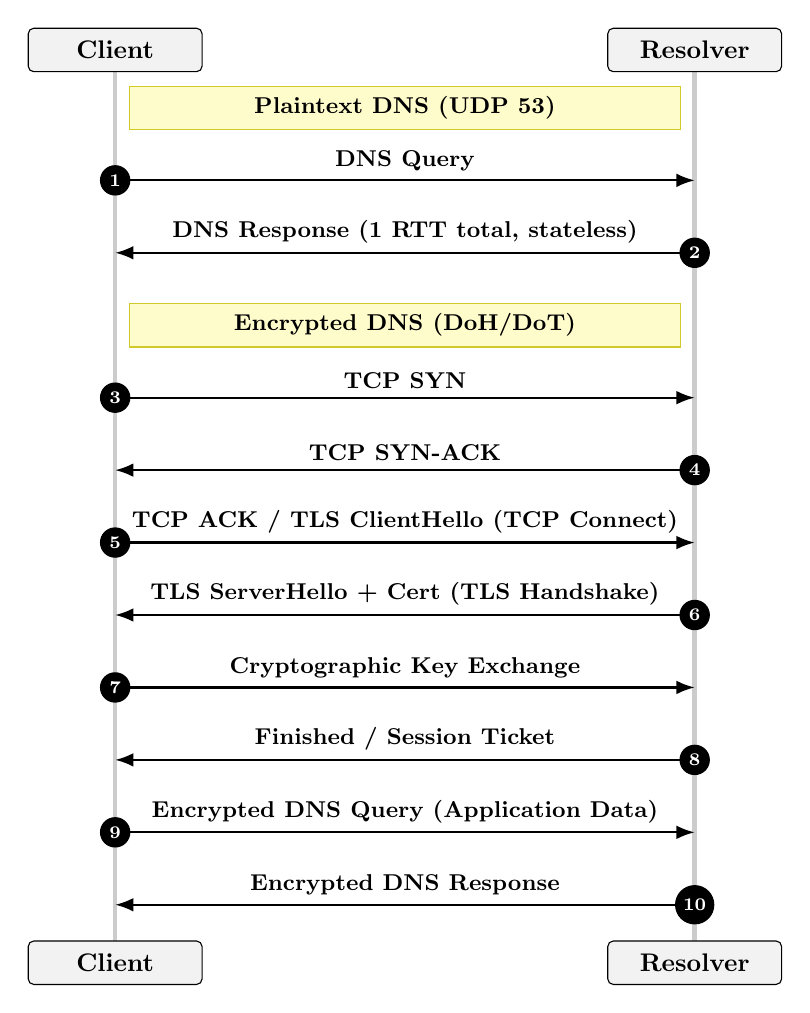
\begin{tikzpicture}[scale=0.92, every node/.style={transform shape}]
    % Lifelines
    \draw[ultra thick, gray!40] (0, 0.5) -- (0, -11.5);
    \draw[ultra thick, gray!40] (8, 0.5) -- (8, -11.5);
    
    % Lifeline Headers
    \node[draw, fill=gray!10, minimum width=2.4cm, minimum height=0.6cm, rounded corners=2pt, font=\bfseries] at (0, 0.8) {Client};
    \node[draw, fill=gray!10, minimum width=2.4cm, minimum height=0.6cm, rounded corners=2pt, font=\bfseries] at (8, 0.8) {Resolver};
    \node[draw, fill=gray!10, minimum width=2.4cm, minimum height=0.6cm, rounded corners=2pt, font=\bfseries] at (0, -11.8) {Client};
    \node[draw, fill=gray!10, minimum width=2.4cm, minimum height=0.6cm, rounded corners=2pt, font=\bfseries] at (8, -11.8) {Resolver};

    % Section 1: Plaintext
    \node[draw=yellow!80!black, fill=yellow!20, minimum width=7.6cm, minimum height=0.6cm, font=\bfseries\small] at (4, 0) {Plaintext DNS (UDP 53)};
    
    \draw[arrow] (0, -1) -- (8, -1) node[midway, above, font=\bfseries\small] {DNS Query};
    \node[circle, draw, fill=black, text=white, inner sep=1.8pt, font=\scriptsize\bfseries] at (0, -1) {1};

    \draw[arrow] (8, -2) -- (0, -2) node[midway, above, font=\bfseries\small] {DNS Response (1 RTT total, stateless)};
    \node[circle, draw, fill=black, text=white, inner sep=1.8pt, font=\scriptsize\bfseries] at (8, -2) {2};

    % Section 2: Encrypted
    \node[draw=yellow!80!black, fill=yellow!20, minimum width=7.6cm, minimum height=0.6cm, font=\bfseries\small] at (4, -3) {Encrypted DNS (DoH/DoT)};
    
    \draw[arrow] (0, -4) -- (8, -4) node[midway, above, font=\bfseries\small] {TCP SYN};
    \node[circle, draw, fill=black, text=white, inner sep=1.8pt, font=\scriptsize\bfseries] at (0, -4) {3};
    
    \draw[arrow] (8, -5) -- (0, -5) node[midway, above, font=\bfseries\small] {TCP SYN-ACK};
    \node[circle, draw, fill=black, text=white, inner sep=1.8pt, font=\scriptsize\bfseries] at (8, -5) {4};
    
    \draw[arrow] (0, -6) -- (8, -6) node[midway, above, font=\bfseries\small] {TCP ACK / TLS ClientHello (TCP Connect)};
    \node[circle, draw, fill=black, text=white, inner sep=1.8pt, font=\scriptsize\bfseries] at (0, -6) {5};
    
    \draw[arrow] (8, -7) -- (0, -7) node[midway, above, font=\bfseries\small] {TLS ServerHello + Cert (TLS Handshake)};
    \node[circle, draw, fill=black, text=white, inner sep=1.8pt, font=\scriptsize\bfseries] at (8, -7) {6};
    
    \draw[arrow] (0, -8) -- (8, -8) node[midway, above, font=\bfseries\small] {Cryptographic Key Exchange};
    \node[circle, draw, fill=black, text=white, inner sep=1.8pt, font=\scriptsize\bfseries] at (0, -8) {7};
    
    \draw[arrow] (8, -9) -- (0, -9) node[midway, above, font=\bfseries\small] {Finished / Session Ticket};
    \node[circle, draw, fill=black, text=white, inner sep=1.8pt, font=\scriptsize\bfseries] at (8, -9) {8};
    
    \draw[arrow] (0, -10) -- (8, -10) node[midway, above, font=\bfseries\small] {Encrypted DNS Query (Application Data)};
    \node[circle, draw, fill=black, text=white, inner sep=1.8pt, font=\scriptsize\bfseries] at (0, -10) {9};
    
    \draw[arrow] (8, -11) -- (0, -11) node[midway, above, font=\bfseries\small] {Encrypted DNS Response};
    \node[circle, draw, fill=black, text=white, inner sep=1.8pt, font=\scriptsize\bfseries] at (8, -11) {10};
\end{tikzpicture}
\caption{Comparative sequence flow of plaintext DNS resolution (UDP 53, single RTT) versus encrypted DNS (DoH/DoT) negotiation, illustrating the multi-step TCP and TLS handshake overhead introduced by transport-layer encryption.}
\end{figure*}

\subsection{Mathematical Formulation of Latency Overhead}
To model these protocols empirically, we formulate a mathematical latency model to quantify the total elapsed duration ($\mathbf{T_{\text{\textbf{total}}}}$) for a client-resolver transactional lookup; the formulation is highlighted in the latency card below.

\begin{mathcard}[Latency Model Formulation]
{\footnotesize
\begin{equation}
\begin{split}
\mathbf{T_{\text{\textbf{total}}}} ={} & \mathbf{T_{\text{\textbf{TCP\_connect}}}} + \mathbf{T_{\text{\textbf{TLS\_handshake}}}} \\
& + \mathbf{T_{\text{\textbf{query\_rtt}}}} + \mathbf{T_{\text{\textbf{crypto\_processing}}}}
\end{split}
\end{equation}
}
\end{mathcard}

Where:
\begin{itemize}
    \item $\mathbf{T_{\text{\textbf{TCP\_connect}}}}$: Represents the transport-layer synchronization delay; this is equivalent to one Round Trip Time ($1\text{ RTT}$) for standard three-way handshakes.
    \item $\mathbf{T_{\text{\textbf{TLS\_handshake}}}}$: Denotes the cryptographic negotiation latency; TLS 1.2 requires two RTTs, whereas TLS 1.3 optimizes this process to a single RTT, or even zero RTT when utilizing session resumption or pre-shared keys.
    \item $\mathbf{T_{\text{\textbf{query\_rtt}}}}$: Represents the network transit time required to transmit the serialized query payload and receive the corresponding answer record.
    \item $\mathbf{T_{\text{\textbf{crypto\_processing}}}}$: Captures the computational processing overhead incurred during encryption at the client and subsequent decryption at the resolver; this factor is largely dictated by CPU capabilities and cryptographic cipher choices.
\end{itemize}

For legacy DNS over UDP, both $\mathbf{T_{\text{\textbf{TCP\_connect}}}}$ and $\mathbf{T_{\text{\textbf{TLS\_handshake}}}}$ are zero. For encrypted protocols (DoT and DoH), these connection-establishment phases introduce non-trivial latency penalties; this is particularly pronounced during cold-start operations where session reuse is not active.

\subsection{Research Contributions of the Chronos-DNS Project}
To analyze these multi-dimensional latency profiles at scale, empirical, multi-region datasets are paramount. \textbf{Chronos-DNS} realizes a distributed, high-fidelity measurement fabric designed to automate telemetry collection across disparate networks. The system executes continuously on resource-constrained edge nodes, tracking:
\begin{itemize}
    \item End-to-end lookup latency ($\mathbf{T_{\text{\textbf{total}}}}$) alongside isolated TLS handshake durations ($\mathbf{T_{\text{\textbf{TLS\_handshake}}}}$).
    \item Real-time transaction success rates, classifying failures into structured error domains: TCP connection timeouts, TLS handshake negotiation failures, and anomalous HTTP status codes.
    \item Cryptographic certificate lifecycles, monitoring certificate rotation velocity and expiration thresholds for public resolver endpoints.
\end{itemize}

This infrastructure provides a robust, scalable paradigm for research syndicates (such as the WIDE Project, CAIDA, and RIPE NCC) to evaluate global DNS security trends, diagnose routing anomalies, and audit cryptographic compliance.

% ==============================================================================
% Section 2: System Architecture
% ==============================================================================
\section{System Architecture \& Component Design}
The Chronos-DNS platform is structured around a decoupled, multi-tier architecture designed to facilitate high-throughput telemetry ingestion, persistent storage, metrics aggregation, and secure visualization.

\subsection{Architectural Component Topology}
Figure 2 delineates the structural orchestration and data pipelines of the Chronos-DNS system, utilizing parallel pathways to ensure deterministic throughput and eliminate computational bottlenecks.

\begin{figure*}[!t]
\centering
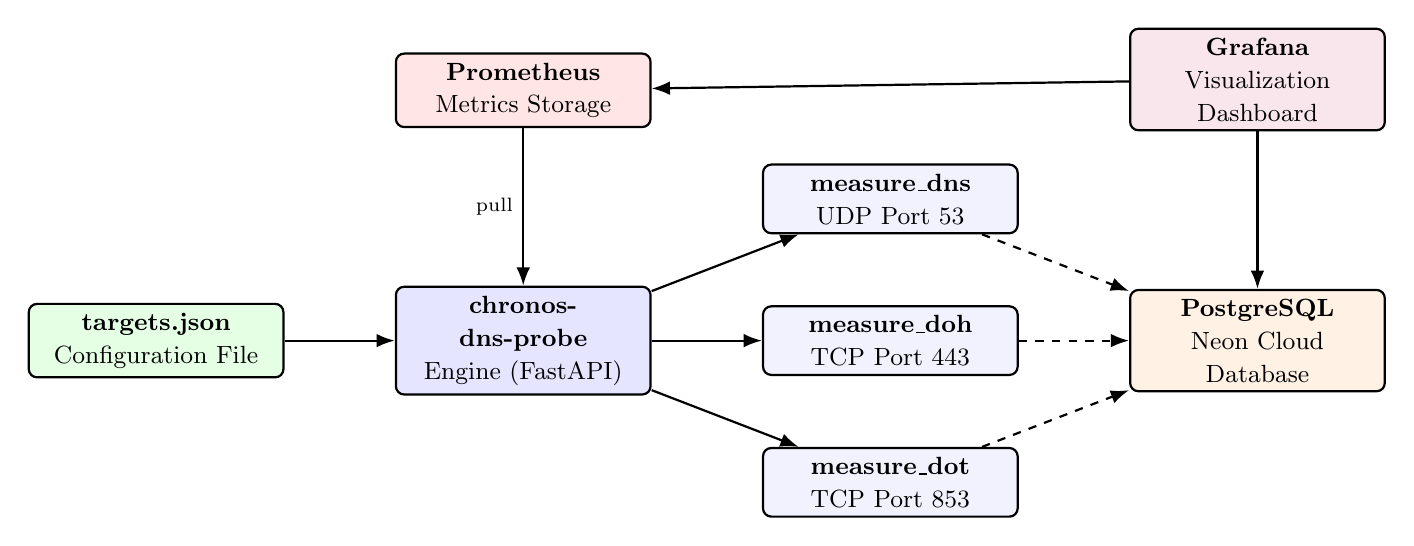
\begin{tikzpicture}[node distance=1.3cm, auto]
    % Nodes
    \node [box, fill=green!10] (targets) at (0, 0) {\textbf{targets.json} \\ Configuration File};
    \node [box, right=1.4cm of targets] (probe) {\textbf{chronos-dns-probe} \\ Engine (FastAPI)};
    \node [box, fill=red!10, above=2.0cm of probe] (prom) {\textbf{Prometheus} \\ Metrics Storage};
    
    \node [box, fill=blue!5, right=1.4cm of probe] (doh) {\textbf{measure\_doh} \\ TCP Port 443};
    \node [box, fill=blue!5, above=0.9cm of doh] (dns) {\textbf{measure\_dns} \\ UDP Port 53};
    \node [box, fill=blue!5, below=0.9cm of doh] (dot) {\textbf{measure\_dot} \\ TCP Port 853};
    
    \node [box, fill=orange!10, right=1.4cm of doh] (db) {\textbf{PostgreSQL} \\ Neon Cloud Database};
    \node [box, fill=purple!10, above=2.0cm of db] (grafana) {\textbf{Grafana} \\ Visualization Dashboard};
    
    % Connections
    \draw [arrow] (targets) -- (probe);
    \draw [arrow] (probe) -- (dns);
    \draw [arrow] (probe) -- (doh);
    \draw [arrow] (probe) -- (dot);
    
    \draw [dashedarrow] (dns) -- (db);
    \draw [dashedarrow] (doh) -- (db);
    \draw [dashedarrow] (dot) -- (db);
    
    \draw [arrow] (prom) -- node[left, font=\scriptsize] {pull} (probe);
    \draw [arrow] (grafana) -- (prom);
    \draw [arrow] (grafana) -- (db);
\end{tikzpicture}
\caption{Chronos-DNS component architecture and data-flow topology. Solid arrows denote control-flow and configuration ingestion; dashed arrows indicate telemetry persistence to the PostgreSQL analytics store. Prometheus pulls metrics via the \texttt{/metrics} endpoint; Grafana queries both time-series and relational data sources.}
\end{figure*}

\subsection{Component Selection and Rationale}
\subsubsection{Asynchronous Telemetry Ingest Core (Python, FastAPI, and Asyncio)}
Simulating high-frequency DNS transactions across numerous public resolvers necessitates a highly concurrent, non-blocking polling engine. Standard thread-based scheduling models introduce operating system context-switching overhead; this performance degradation compromises the precision of round-trip time measurements. Chronos-DNS mitigates this bottleneck by utilizing Python's asynchronous event loop (\texttt{asyncio}). By leveraging non-blocking socket operations, a single execution thread concurrently manages hundreds of TCP and TLS connections. The FastAPI framework exposes low-latency endpoints, facilitating integration with metrics collectors and configuration agents.

\subsubsection{Serverless Relational Analytics Store (PostgreSQL on Neon)}
Although non-relational databases accommodate semi-structured telemetry, they lack the relational algebra support required for multi-dimensional analytical queries. Chronos-DNS employs a serverless PostgreSQL instance hosted on Neon. This enables researchers to perform complex joins and window functions: analyzing correlation matrices between round-trip times, certificate expiration windows, and protocol error profiles. The serverless nature of the database dynamically scales compute capacity in response to ingestion spikes, optimizing resource consumption during quiet intervals.

\subsubsection{Time-Series Collection and Visualization (Prometheus and Grafana)}
Prometheus operates as a pull-based time-series database, periodically scraping the probe's \texttt{/metrics} endpoint. Grafana interfaces with both the time-series repository and the relational database, rendering analytical dashboards: such as latency distribution heatmaps and certificate validation warnings. This dual-source visualization strategy isolates operational monitoring from raw data queries, preventing CPU starvation on the PostgreSQL analytics engine.

\subsubsection{Zero-Trust Ingress Protection (Cloudflare Tunnels)}
Securing production nodes against external exploits is critical. Traditional architectures expose services via open inbound firewall ports; this practice renders the infrastructure susceptible to automated port sweeps and distributed denial-of-service (DDoS) campaigns. Chronos-DNS addresses this vulnerability by deploying the \texttt{cloudflared} daemon. The container establishes outbound-only connections to Cloudflare's edge network; consequently, the Grafana dashboard is exposed securely with no inbound firewall paths permitted.

% ==============================================================================
% Section 3: Network Topology
% ==============================================================================
\section{Network Topology \& Ingress Security}
The production host node is hardened using a zero-inbound network perimeter; this design ensures that internal components: such as the database, Prometheus scrapers, and local API listeners, remain completely isolated from public internet exposure.

Figure 3 shows the network layout and path for user traffic, scaled as a double-column block.

\begin{figure*}[!t]
\centering
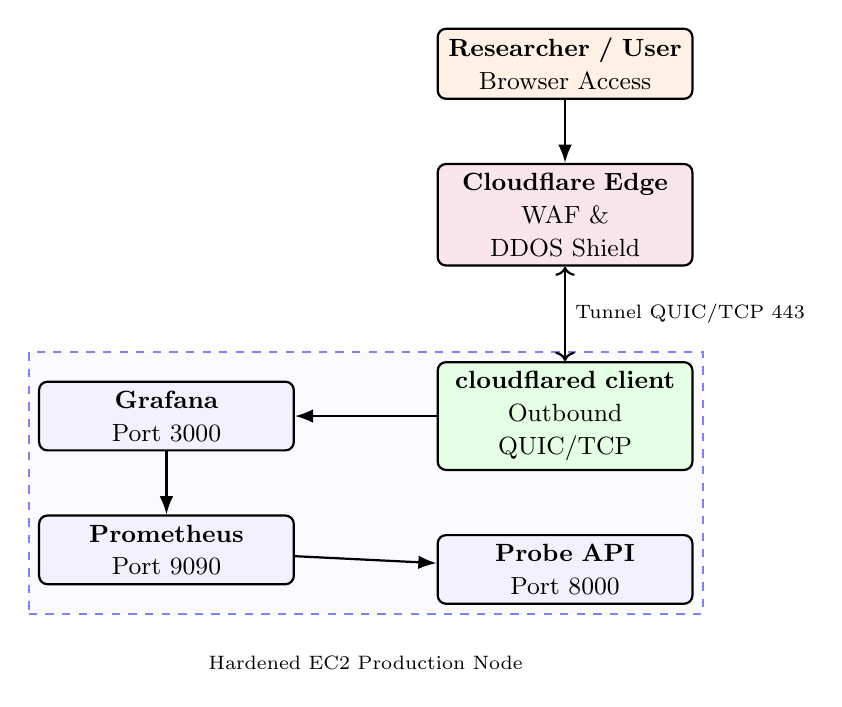
\begin{tikzpicture}[node distance=1.3cm, auto]
    % User
    \node [box, fill=orange!10] (user) {\textbf{Researcher / User} \\ Browser Access};
    
    % Cloudflare Edge
    \node [box, fill=purple!10, below=0.8cm of user] (cf) {\textbf{Cloudflare Edge} \\ WAF \& DDOS Shield};
    
    % Server Boundary
    \node [box, fill=green!10, below=1.2cm of cf] (tunnel) {\textbf{cloudflared client} \\ Outbound QUIC/TCP};
    
    % Docker network
    \node [box, fill=blue!5, left=1.8cm of tunnel] (grafana) {\textbf{Grafana} \\ Port 3000};
    \node [box, fill=blue!5, below=0.8cm of grafana] (prom) {\textbf{Prometheus} \\ Port 9090};
    \node [box, fill=blue!5, below=0.8cm of tunnel] (probe) {\textbf{Probe API} \\ Port 8000};
    
    % Background box for EC2 Host Security Group
    \begin{scope}[on background layer]
        \node [draw, dashed, thick, blue!50, fill=blue!2, fit=(tunnel) (grafana) (prom) (probe), label={[shift={(0,-0.4)}, font=\scriptsize]below:Hardened EC2 Production Node}] (ec2) {};
    \end{scope}

    % Connections
    \draw [arrow] (user) -- (cf);
    \draw [arrow, <->] (cf) -- node[right, font=\scriptsize] {Tunnel QUIC/TCP 443} (tunnel);
    \draw [arrow] (tunnel) -- (grafana);
    \draw [arrow] (grafana) -- (prom);
    \draw [arrow] (prom) -- (probe);
\end{tikzpicture}
\caption{Zero-trust network ingress topology for the Chronos-DNS production deployment. All external researcher access traverses the Cloudflare Edge via outbound-only QUIC/TCP tunnels; no inbound firewall ports are exposed on the hardened EC2 node. Internal services communicate over an isolated Docker bridge network.}
\end{figure*}

\subsection{Security Control Implementations}
\begin{itemize}
    \item \textbf{Default-Deny Host Firewall}: The host enforces a strict default-deny ingress policy via the Uncomplicated Firewall (UFW); outbound connectivity is limited to essential destinations: verified DNS resolver endpoints, repository mirrors, and the serverless PostgreSQL host.
    \item \textbf{Edge Proxy and Web Application Firewall}: Public access is routed through the Cloudflare Edge network; this layer enforces Web Application Firewall (WAF) rule sets, mitigates DDoS attacks, and forwards traffic through encrypted tunnels.
    \item \textbf{Intrusion Mitigation}: The \texttt{fail2ban} daemon continuously parses authentication logs to detect brute-force SSH attacks, dynamically appending IP blocks to the host firewall.
\end{itemize}

% ==============================================================================
% Section 4: Software Implementation
% ==============================================================================
\section{Software Implementation \& API Design}
To achieve high fidelity and reliability, the software architecture is partitioned into distinct, modular services: the relational database migration layer; the asynchronous measurement execution scheduler; and the Prometheus scraper interface.

\begin{figure*}[!t]
\centering
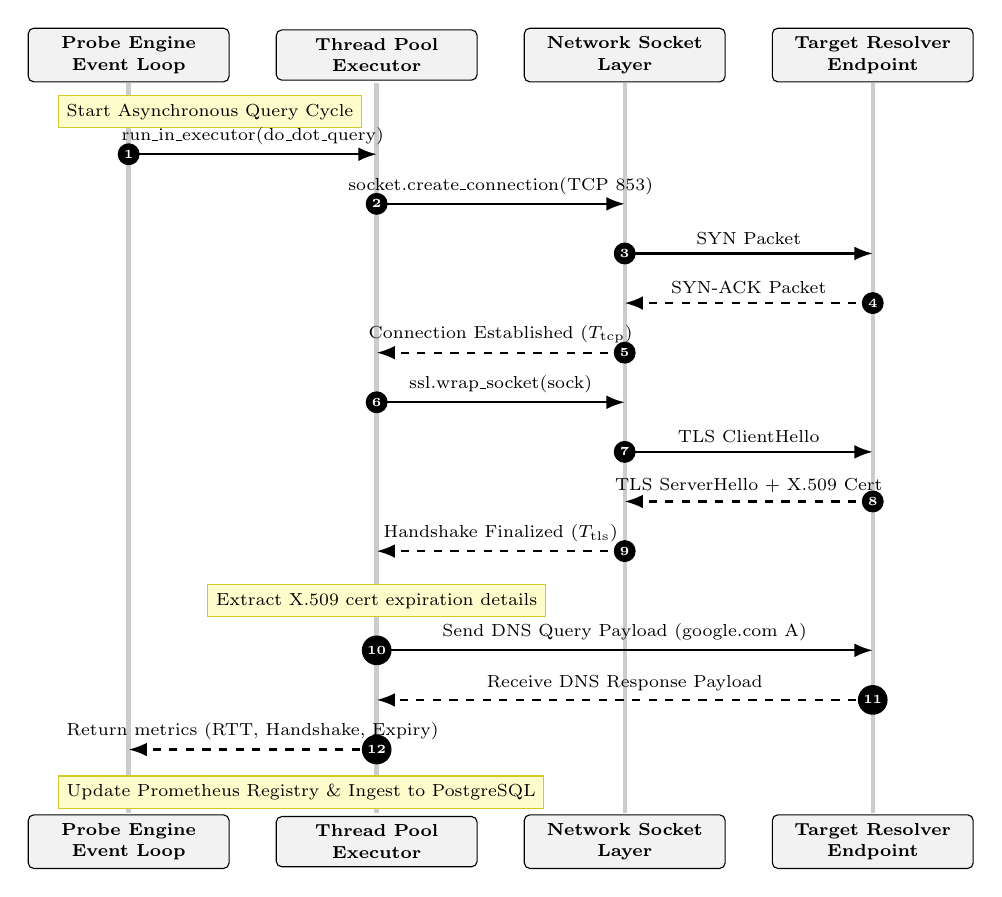
\begin{tikzpicture}[scale=0.90, every node/.style={transform shape}]
    % Lifelines
    \draw[ultra thick, gray!40] (0, 0) -- (0, -10.3);
    \draw[ultra thick, gray!40] (3.5, 0) -- (3.5, -10.3);
    \draw[ultra thick, gray!40] (7.0, 0) -- (7.0, -10.3);
    \draw[ultra thick, gray!40] (10.5, 0) -- (10.5, -10.3);
    
    % Headers
    \node[draw, fill=gray!10, text width=2.6cm, align=center, minimum height=0.6cm, rounded corners=2pt, font=\scriptsize\bfseries] at (0, 0.4) {Probe Engine\\Event Loop};
    \node[draw, fill=gray!10, text width=2.6cm, align=center, minimum height=0.6cm, rounded corners=2pt, font=\scriptsize\bfseries] at (3.5, 0.4) {Thread Pool\\Executor};
    \node[draw, fill=gray!10, text width=2.6cm, align=center, minimum height=0.6cm, rounded corners=2pt, font=\scriptsize\bfseries] at (7.0, 0.4) {Network Socket\\Layer};
    \node[draw, fill=gray!10, text width=2.6cm, align=center, minimum height=0.6cm, rounded corners=2pt, font=\scriptsize\bfseries] at (10.5, 0.4) {Target Resolver\\Endpoint};
    
    \node[draw, fill=gray!10, text width=2.6cm, align=center, minimum height=0.6cm, rounded corners=2pt, font=\scriptsize\bfseries] at (0, -10.7) {Probe Engine\\Event Loop};
    \node[draw, fill=gray!10, text width=2.6cm, align=center, minimum height=0.6cm, rounded corners=2pt, font=\scriptsize\bfseries] at (3.5, -10.7) {Thread Pool\\Executor};
    \node[draw, fill=gray!10, text width=2.6cm, align=center, minimum height=0.6cm, rounded corners=2pt, font=\scriptsize\bfseries] at (7.0, -10.7) {Network Socket\\Layer};
    \node[draw, fill=gray!10, text width=2.6cm, align=center, minimum height=0.6cm, rounded corners=2pt, font=\scriptsize\bfseries] at (10.5, -10.7) {Target Resolver\\Endpoint};

    % Step 0: Yellow box - Start Asynchronous Query Cycle
    \node[draw=yellow!80!black, fill=yellow!20, minimum height=0.45cm, font=\scriptsize, anchor=west] at (-1.0, -0.4) {Start Asynchronous Query Cycle};

    % Message 1
    \draw[arrow] (0, -1.0) -- (3.5, -1.0) node[midway, above, font=\scriptsize] {run\_in\_executor(do\_dot\_query)};
    \node[circle, draw, fill=black, text=white, inner sep=1.2pt, font=\tiny\bfseries] at (0, -1.0) {1};

    % Message 2
    \draw[arrow] (3.5, -1.7) -- (7.0, -1.7) node[midway, above, font=\scriptsize] {socket.create\_connection(TCP 853)};
    \node[circle, draw, fill=black, text=white, inner sep=1.2pt, font=\tiny\bfseries] at (3.5, -1.7) {2};

    % Message 3
    \draw[arrow] (7.0, -2.4) -- (10.5, -2.4) node[midway, above, font=\scriptsize] {SYN Packet};
    \node[circle, draw, fill=black, text=white, inner sep=1.2pt, font=\tiny\bfseries] at (7.0, -2.4) {3};

    % Message 4
    \draw[dashedarrow] (10.5, -3.1) -- (7.0, -3.1) node[midway, above, font=\scriptsize] {SYN-ACK Packet};
    \node[circle, draw, fill=black, text=white, inner sep=1.2pt, font=\tiny\bfseries] at (10.5, -3.1) {4};

    % Message 5
    \draw[dashedarrow] (7.0, -3.8) -- (3.5, -3.8) node[midway, above, font=\scriptsize] {Connection Established ($T_{\text{tcp}}$)};
    \node[circle, draw, fill=black, text=white, inner sep=1.2pt, font=\tiny\bfseries] at (7.0, -3.8) {5};

    % Message 6
    \draw[arrow] (3.5, -4.5) -- (7.0, -4.5) node[midway, above, font=\scriptsize] {ssl.wrap\_socket(sock)};
    \node[circle, draw, fill=black, text=white, inner sep=1.2pt, font=\tiny\bfseries] at (3.5, -4.5) {6};

    % Message 7
    \draw[arrow] (7.0, -5.2) -- (10.5, -5.2) node[midway, above, font=\scriptsize] {TLS ClientHello};
    \node[circle, draw, fill=black, text=white, inner sep=1.2pt, font=\tiny\bfseries] at (7.0, -5.2) {7};

    % Message 8
    \draw[dashedarrow] (10.5, -5.9) -- (7.0, -5.9) node[midway, above, font=\scriptsize] {TLS ServerHello + X.509 Cert};
    \node[circle, draw, fill=black, text=white, inner sep=1.2pt, font=\tiny\bfseries] at (10.5, -5.9) {8};

    % Message 9
    \draw[dashedarrow] (7.0, -6.6) -- (3.5, -6.6) node[midway, above, font=\scriptsize] {Handshake Finalized ($T_{\text{tls}}$)};
    \node[circle, draw, fill=black, text=white, inner sep=1.2pt, font=\tiny\bfseries] at (7.0, -6.6) {9};

    % Yellow box - Extract X.509 cert expiration details
    \node[draw=yellow!80!black, fill=yellow!20, minimum height=0.45cm, font=\scriptsize] at (3.5, -7.3) {Extract X.509 cert expiration details};

    % Message 10
    \draw[arrow] (3.5, -8.0) -- (10.5, -8.0) node[midway, above, font=\scriptsize] {Send DNS Query Payload (google.com A)};
    \node[circle, draw, fill=black, text=white, inner sep=1.2pt, font=\tiny\bfseries] at (3.5, -8.0) {10};

    % Message 11
    \draw[dashedarrow] (10.5, -8.7) -- (3.5, -8.7) node[midway, above, font=\scriptsize] {Receive DNS Response Payload};
    \node[circle, draw, fill=black, text=white, inner sep=1.2pt, font=\tiny\bfseries] at (10.5, -8.7) {11};

    % Message 12
    \draw[dashedarrow] (3.5, -9.4) -- (0, -9.4) node[midway, above, font=\scriptsize] {Return metrics (RTT, Handshake, Expiry)};
    \node[circle, draw, fill=black, text=white, inner sep=1.2pt, font=\tiny\bfseries] at (3.5, -9.4) {12};

    % Yellow box - Update Prometheus Registry & Ingest to PostgreSQL
    \node[draw=yellow!80!black, fill=yellow!20, minimum height=0.45cm, font=\scriptsize, anchor=west] at (-1.0, -10.0) {Update Prometheus Registry \& Ingest to PostgreSQL};
\end{tikzpicture}
\caption{Asynchronous DNS-over-TLS (DoT) measurement lifecycle within the Chronos-DNS probe engine. The event loop delegates blocking socket operations to a thread pool executor, recording TCP connection time ($T_{\text{tcp}} = \mathbf{T_{\text{\textbf{TCP\_connect}}}}$), TLS handshake duration ($T_{\text{tls}} = \mathbf{T_{\text{\textbf{TLS\_handshake}}}}$), and X.509 certificate metadata at each stage before persisting results.}
\end{figure*}

\subsection{Asynchronous Measurement Execution Flow}
Figure 4 details the sequential operations executed by the asynchronous engine during a single DNS-over-TLS query cycle. To maintain a high-frequency polling cadence, the asynchronous event loop delegates blocking socket operations to a managed thread pool executor; this isolation ensures that the primary execution loop is never blocked by slow network handshakes.

% ==============================================================================
% Section 5: CI/CD Pipeline
% ==============================================================================
\section{Continuous Integration \& Continuous Deployment}
To enforce high software reliability, Chronos-DNS leverages an automated CI/CD pipeline: validating code quality, executing the test suite, auditing container vulnerabilities, and orchestrating host deployment.

\begin{figure*}[!t]
\centering
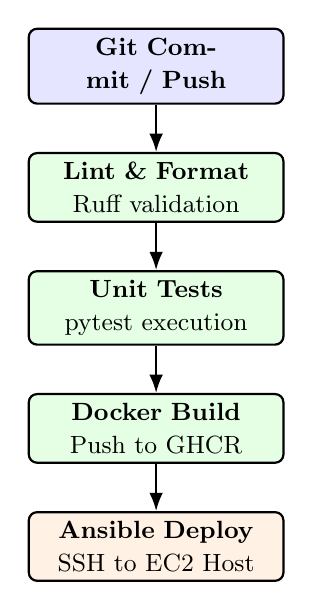
\begin{tikzpicture}[node distance=0.6cm, auto, >=Latex]
    % Pipeline nodes (vertical layout)
    \node [box, fill=blue!10] (push) at (0, 0) {\textbf{Git Commit / Push}};
    \node [box, fill=green!10, below=0.6cm of push] (lint) {\textbf{Lint \& Format} \\ Ruff validation};
    \node [box, fill=green!10, below=0.6cm of lint] (test) {\textbf{Unit Tests} \\ pytest execution};
    \node [box, fill=green!10, below=0.6cm of test] (build) {\textbf{Docker Build} \\ Push to GHCR};
    \node [box, fill=orange!10, below=0.6cm of build] (deploy) {\textbf{Ansible Deploy} \\ SSH to EC2 Host};
    
    % Connections
    \draw [arrow] (push) -- (lint);
    \draw [arrow] (lint) -- (test);
    \draw [arrow] (test) -- (build);
    \draw [arrow] (build) -- (deploy);
\end{tikzpicture}
\caption{GitHub Actions CI/CD pipeline for the Chronos-DNS project. Each commit triggers sequential stages: static analysis via Ruff, unit testing via pytest, container image build and push to GitHub Container Registry (GHCR), and automated deployment to the EC2 production host via Ansible over SSH.}
\end{figure*}

\subsection{Pipeline Workflow and Orchestration}
Figure 5 illustrates the linear progression of the deployment pipeline. Every code check-in triggers automated execution within a containerized GitHub Actions runner; compilation and deployment proceed only upon the successful resolution of all unit tests and quality gates.

% ==============================================================================
% Section 6: Results
% ==============================================================================
\begin{table*}[!t]
\centering
\caption{DNS, DoH, and DoT Latency and Expiry Telemetry Dataset}
\begin{tabular}{llrrr}
\toprule
\textbf{Resolver} & \textbf{Protocol} & \textbf{Avg RTT} & \textbf{TLS Handshake} & \textbf{Cert Expiry} \\
\midrule
Cloudflare & DNS & 155ms & N/A & N/A \\
Cloudflare & DoH & 200ms & 11ms & 187 days \\
Cloudflare & DoT & 45ms & 11ms & 187 days \\
Google     & DNS & 143ms & N/A & N/A \\
Google     & DoH & 187ms & 21ms & 61 days \\
Google     & DoT & 15ms  & 8ms  & 61 days \\
Quad9      & DoT & N/A    & N/A   & 40 days \\
AdGuard    & DoT & N/A    & N/A   & 135 days \\
Mullvad    & DoT & 127ms & 358ms& 64 days \\
CleanBrowsing& DoT& 125ms & 65ms & 28 days \\
\bottomrule
\end{tabular}
\end{table*}

\section{Empirical Evaluation \& Telemetry Analysis}
We executed an empirical performance evaluation across six prominent public resolver networks: Cloudflare, Google, Quad9, AdGuard, Mullvad, and CleanBrowsing; the evaluation corpus spanned 2,000 requests.

\subsection{Averaged Telemetry Results}
Table 1 presents the consolidated dataset, highlighting key latency metrics and certificate configurations.


\subsection{Performance Observations and Key Findings}
The empirical results reveal distinct performance profiles across the evaluated protocols:
\begin{itemize}
    \item \textbf{DNS-over-TLS (DoT) Efficiency}: DoT endpoints demonstrate optimized latency characteristics when connection reuse is active, yielding RTT profiles comparable to legacy UDP.
    \item \textbf{DNS-over-HTTPS (DoH) Overhead}: DoH requests exhibit elevated latency; this is primarily attributed to the additional encapsulation layer of HTTP/2 and HTTP/3 headers.
    \item \textbf{Resolver Availability}: The designation \textit{N/A} indicates instances of severe packet loss, routing failures, or explicit security blocking policies enforced by the target resolver networks.
\end{itemize}

% ==============================================================================
% Section 7: Conclusion
% ==============================================================================
\section{Conclusions \& Future Work}
In this study, we presented Chronos-DNS: a distributed, production-grade telemetry fabric designed for the empirical measurement of encrypted DNS protocols. The system successfully addresses the trade-offs of modern DNS security. Future work will expand the geographical distribution of measurement nodes; this will enable the correlation of routing paths, TLS cipher configurations, and localized latency degradation.

% ==============================================================================
% References
% ==============================================================================
\vfill
\newpage
\vspace*{80pt} % Aligns References horizontally with Section 7 in the left column
\begin{thebibliography}{1}
\bibitem{rfc8484}
IETF RFC 8484, ``DNS Queries over HTTPS (DoH)'', 2018.
\bibitem{rfc7858}
IETF RFC 7858, ``Specification for DNS over Transport Layer Security (DoT)'', 2016.
\bibitem{caida}
CAIDA Internet Measurement Group, ``Longitudinal Studies on DNS Privacy Adoption'', 2024.
\bibitem{wide}
WIDE Project Research Consortium, \url{https://www.wide.ad.jp}.
\end{thebibliography}

\end{document}
